\chapter{Preface}
This thesis is submitted in partial fulfilment of the requirements for the degree of Master of Science in Applied Physics and Mathematics: Industrial Mathematics.
It concludes five-ish years in the moustache city and somewhat more at Norges tekniske høiskole.
It has certainly been one of the periods in my life.

I would like to thank my external supervisors from Sintef, Frank Georg Fuchs and Alexander Stasik, for their continuous guidance and support, for suggesting a great topic for the thesis, for their time and for giving me, who had no prior experience with quantum computing, the opportunity to learn about it.
Prior to the thesis, I had no idea about what to write, so the immediate support and encouragement, as well as the mere opportunity to study something interesting, are something for which I am grateful.
Furthermore, I also want to thank my internal supervisor, Gunnar Taraldsen, for our regular meetings in which I was forced into thinking more critically about what I was writing, for letting me write about something special and for still caring about my project despite venturing into a novel field partly outside his wide expertise.

\makebox[\dimexpr\textwidth-\parindent][s]{Do note that this master's thesis is based}
on the preparatory specialisation project report~\autocite{sjo2022}, carried out in the previous semester, the autumn of 2022.
The theory of artificial neural networks, quantum computing and quantum machine learning, in addition to parts of the introduction, are mostly taken from the report.
Particularly \cref{sec:nn,sec:qstates,sec:quantum_operations,sec:nisq,sec:vqa,sec:qnn} are lifted directly thence with only minor modifications to the text.

\vspace*{0.5cm}
\begin{figure}[h]
  \raggedleft
  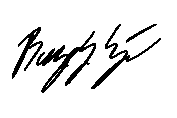
\includegraphics[width=0.3\linewidth]{blank.pdf}
\end{figure}
\begin{flushright}
  \vspace{-1.3cm}
  Boye Gravningen Sjo \\
  Trondhjem, Norge \\
  12th of June, 2023
\end{flushright}

\cleardoublepage